\chapter{Desenvolvimento}

Este capítulo descreve conceitualmente a solução implementada, detalhando o fluxo de dados, a arquitetura do sistema e os componentes de software que o compõem. O objetivo aqui é descrever como os conceitos foram traduzidos em código e estrutura de software, detalhando a organização do repositório de código, o funcionamento interno dos principais módulos desenvolvidos em Python e, por fim, apresentando um estudo de caso para ilustrar a aplicação prática da arquitetura em um pipeline específico.

\section{Arquitetura geral e fluxo de dados}

Para solucionar o problema da complexidade e descentralização dos dados, foi projetada e desenvolvida uma arquitetura de software robusta, focada em automação, modularidade e escalabilidade. A metodologia adotada buscou o desacoplamento de responsabilidades e a configuração declarativa, permitindo que o sistema seja flexível e de fácil manutenção.

A solução opera em um sistema de processamentos de dados em lote. O fluxo de informações foi desenhado seguindo um modelo de sepração entre camadas, conforme ilustrado na Figura\ref{fig:diagrama} e descritos nos passos abaixos: 

\begin{figure}[H]
  \centering
  \caption{Diagrama do projeto}\label{fig:diagrama}
  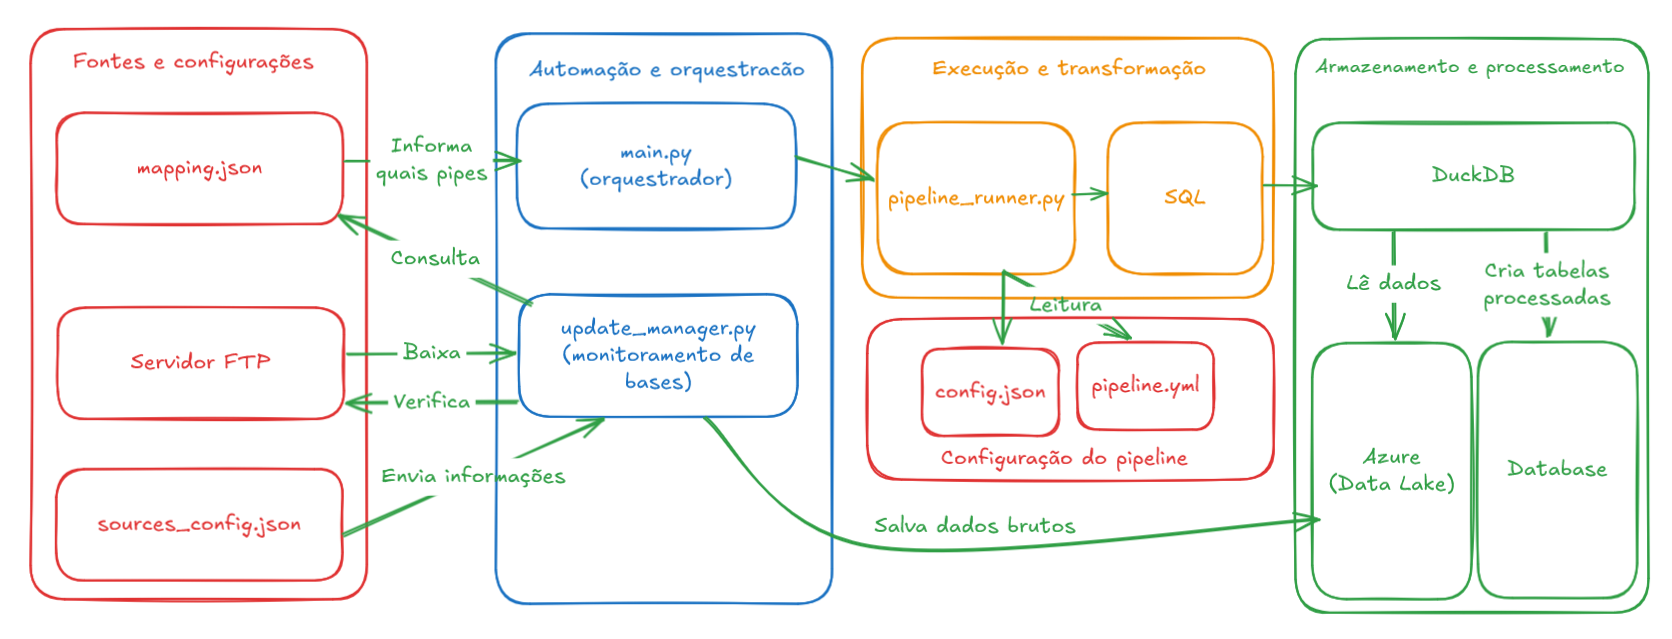
\includegraphics[width=1\linewidth]{imagens/diagrama.png}
  \par
  \footnotesize{Fonte: Documentos da empresa.}
\end{figure}

\subsection{Fontes e configurações}

A parte inicial do sistema são as fontes de dados externa, que são acessadas através dos servidores FTP do DATASUS e da ANS, onde são disponibilizados os arquivos públicos.

Os arquivos de configuração, acessados pelos orquestradores, contém informações essenciais para o pipeline. Através do $sources\_config.json$, obtemos todos os detalhes principais de cada fonte, e última vez que atualizamos esta base de dados. O $mapping.json$ é encarregado de informar quais fontes cada pipeline utiliza, para que possamos processar apenas os que tiveram uma fonte atualizada.

\subsection{Automação e orquestração}

Foi configurado para que o ciclo de processamento seja iniciado de forma autônoma duas vezes por més através do $update\_manager.py$, o agente que monitora continuamente as fontes de dados. Ao detectar um arquivo novo, é verificado quais pipelines serão processados, e em seguida realizado a chamada do $main.py$ para executar o orquestramento de cada um.

\subsection{Configuração do pipeline}

Cada pipeline é definido com um conjunto de arquivos de configuração. O $pipeline.yml$ atua como uma receita, onde especifica quais fontes devem ser lidas, a sequências de transformações em SQL a serem aplicadas e as tabelas finais a serem salvas.
Enquanto o  $config.json$, detalha os aspectos técnicos de cada fonte, como o caminho bruto no Azure, delimitador e codificação de caracteres.

\subsection{Execução e transformação}

Quando iniciado, o $pipeline\_runner.py$ assume a execução. Através do DuckDB, ele é reponsável por ler os dados diretamente da camada bruta do Azure, a lógica da transformação contida nos scripts SQL, e então, executada em memória. Esta fase é a responsável pela limpeza, padronização, junção e enriquecimento dos dados.

\subsection{Armazenamento e processamento}

O motor de processamento é o DuckDB, escolhido pela alta performance em cargas grandes de trabalho. O armazenamento é gerenciado pelo Azure Blob Stora, que funciona como um Data Warehouse. No final do fluxo, os dados processados são carregados para o Azure, onde ficam disponívems em um formato otimizado para consumo por aplicações analíticas e pela plataforma de inteligência de mercado da LifesHub.

\section{Estrutura do repositório do código}

Para garantir a modularidade, manutenibilidade e a clareza do projeto, o código-fonte foi organizado em uma estrutura baseada em diretórios com cada módulo tendo sua responsabilidade definida, conforme ilustrado na Figura \ref{fig:repo}.

\begin{figure}[H]
  \centering
  \caption{Diagrama do projeto}\label{fig:repo}
  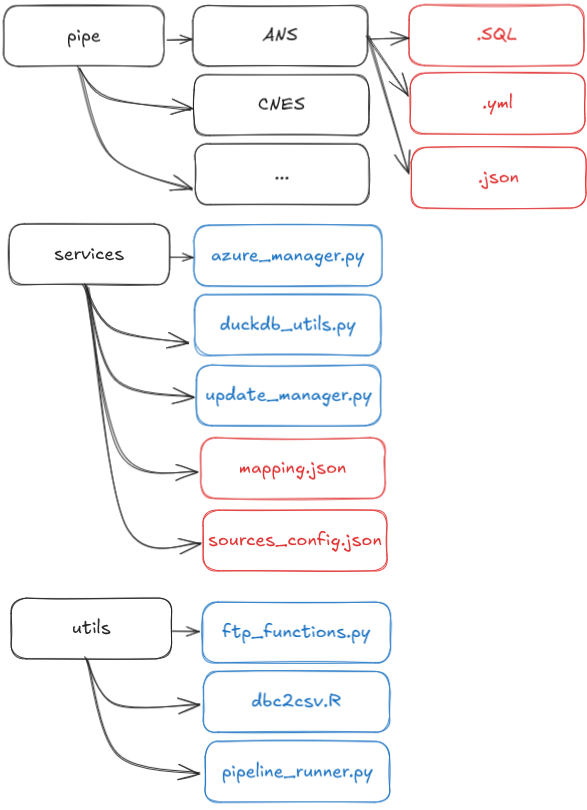
\includegraphics[width=.5\linewidth]{imagens/repo.png}
  \par
  \footnotesize{Fonte: Documentos da empresa.}
\end{figure}

\begin{itemize}
    \item \textbf{/pipe:} Contém todos os pipelines do projeto com seus respectivos arquivos de configuração, \texttt{config.json} e \texttt{pipeline.yml}, e os scripts \texttt{.sql}. Cada subdiretório corresponde a um fluxo (ex: \texttt{/ans/beneficiarios})
    
    \item \textbf{/services:} Abriga os módulos que interagem com serviços externos, \texttt{duckdb\_utils.py} e \texttt{azure\_manager.py}, ou funções de alto nível, como o \texttt{update\_manager.py} (bot)
    
    \item \textbf{/utils:} Arquivos utilitários para o funcionamento do projeto. Essenciais para o framework do pipeline, como a conexão com os servidores FTP, o conversor de \.dbc para \.csv, o orquestrador do pipeline e outros arquivos.
\end{itemize}

\section{Implementação dos componentes}



\section{Estudo de caso}